% PVLDB Volume 20, Scalable Data Science category (8 pages plus references).
% Build: pdflatex main; bibtex main; pdflatex main; pdflatex main
\documentclass[sigconf, nonacm]{acmart}
%%% VLDB block start %%%
\usepackage{pvldb}
%%% VLDB block end %%%
\renewcommand\vldbdoi{XX.XX/XXX.XX}
\renewcommand\vldbpages{XXX-XXX}
\renewcommand\vldbavailabilityurl{https://github.com/ahb-sjsu/turboquant-pro/tree/master/benchmarks/fleet}

\usepackage{booktabs}
\usepackage{pgfplots}
\pgfplotsset{compat=1.18}
\usepgfplotslibrary{statistics}

\begin{document}
\title{Recall Does Not Move at a Trillion Rows}
\subtitle{Routed search over compressed vectors, measured against the exact scan, on a shared research cluster}

\author{Andrew H. Bond}
\orcid{0009-0003-2599-6158}
\affiliation{%
  \institution{San Jos\'e State University}
  \city{San Jos\'e}
  \state{California}
  \country{USA}
}
\email{andrew.bond@sjsu.edu}

\begin{abstract}
We report a measurement of routed inverted-file search over an index of one trillion 4-bit
product-quantized vectors, built and queried on a shared, policy-enforced Kubernetes research
cluster with no dedicated hardware. The index is 500 servers of two billion rows each, 24.0 bytes
per row, 24 TB in all, on one block volume per server. Against the exact full scan of the same
compressed index, routed search returns recall at ten of 0.989 when it probes 32 of 2048 cells and
0.999 when it probes 128, on 100 queries. The same protocol gave 0.979 and 0.999 at one hundred
million rows, 0.982 and 0.999 at ten billion, and 0.983 and 0.999 at one hundred billion. Recall
against the full scan does not move across four orders of magnitude of corpus size. The result is
a self-consistency measure on a synthetic corpus of low intrinsic dimension, and we state what it
does and does not license. The second contribution is the run itself. Every job ran in the
cluster's enforcement-exempt class of one CPU and two gigabytes, which three failed pilots showed
requires reading the query set from a cache, holding at most two memory-mapped shards open, and
scanning in blocks of 65536 rows. A pool driver with idempotent per-server jobs, exponential
back-off, and a rule that a job the controller has deferred is not a job that vanished carried
928 submissions to 849 completions with no operator restart, across one host that killed every
job placed on it and three nodes that went unreachable mid-scan. The reference scan cost 418
CPU-hours and the two routed passes 354. Every log, state file, partial result and the score are
in the repository.
\end{abstract}

\maketitle

\section{Introduction}

Approximate nearest-neighbour search over compressed vectors is now routine at a billion rows
\cite{jegou2011product,johnson2019faiss,chen2021spann}. The question this paper answers is
narrower than most and, we think, worth answering on its own. When an inverted-file index is
partitioned into shards that share one coarse quantizer and one rotation, and the corpus grows by
adding shards rather than by densifying old ones, does the routing lose anything it would have
found by scanning everything? The honest way to ask it is to build the whole index, scan the whole
index exactly, and compare. We did that at one trillion rows.

The setting matters as much as the number. The index was built and measured on the National
Research Platform's Nautilus cluster, a Kubernetes federation shared by dozens of groups, where
resource requests are policed by an enforcer that deletes pods whose usage falls outside a band
around their request, and where the only class of workload that is never touched is one CPU and
two gigabytes of memory. There is no reserved partition, no InfiniBand, and no guarantee that a
node that accepted a pod will still be reachable an hour later. A measurement at this scale on
such a platform is a data-engineering problem before it is a retrieval problem, and the second
half of the paper is about that problem.

The paper makes three claims and one disclaimer.

\begin{itemize}
\item Routed recall against the exact scan of the same index is 0.989 at 32 probes and 0.999 at 128
probes at $10^{12}$ rows, and the same protocol at $10^{8}$, $10^{10}$ and $10^{11}$ rows gave
figures within 0.01 of these at 32 probes and within 0.001 at 128 probes (Section~\ref{sec:results}).
\item Every phase of the measurement fits the cluster's exempt envelope of one CPU and two
gigabytes once three memory paths are closed, each of which a pilot found by dying
(Section~\ref{sec:shape}).
\item A pool driver built on idempotent jobs and a small number of explicit failure rules finishes
a two-day, 928-submission run on a shared cluster without an operator, and we report every rule
and every failure class with counts (Section~\ref{sec:pool}).
\item The disclaimer is that the corpus is synthetic, of intrinsic dimension about 16, and the
recall reported is against the compressed index's own exact scan rather than against float ground
truth. Section~\ref{sec:limits} gives the numbers that bound what the result means, including a
real-embedding pilot on which the same routing holds but the compression itself does not.
\end{itemize}

\section{The index and the corpus}
\label{sec:system}

\paragraph{Index.} Each row is a 32-dimensional vector projected to 24 dimensions by one PCA
basis shared by the whole fleet, quantized to 4 bits per dimension, and assigned to one of 2048
inverted-file cells by one shared coarse quantizer. A shard holds five million rows. A server
holds 400 shards, two billion rows, on one block volume. The on-disk row is 12 bytes of codes, 8
bytes of per-row norms used by the asymmetric distance computation, and 4 bytes of cell
membership, 24.0 bytes measured. Scoring is asymmetric distance computation over the codes, in
row blocks, from memory-mapped shards. Because the basis and the coarse quantizer are shared,
scores from different shards are comparable and a global top-$k$ is the exact merge of per-shard
top-$k$s. That property is what makes the measurement below exact rather than approximate.

\paragraph{Corpus.} The corpus is defined by a seed and regenerated on demand, so the distributed
build moves no corpus bytes. Each global shard draws a fresh rank-16 Gaussian basis, projects
Gaussian coefficients through it with a linear decay of singular values from 1.0 to 0.3, and adds
five percent noise, in an ambient dimension of 32. Its intrinsic dimension measures 15.4 to 17.0
at every size we tested and does not move with row count. Real embeddings such as Cohere Embed v3
at 1024 dimensions measure 52 to 61 by the same estimator. Hubness, the concentration of
nearest-neighbour lists on a few points, does rise with corpus size on this recipe, at about 0.42
per decade at $k=10$ against roughly 0.25 per decade on real data, because random 16-dimensional
subspaces of a 32-dimensional space overlap. The corpus therefore gets harder in one respect as it
grows and the recall reported below holds despite that.

\paragraph{Scale points.} The same protocol has been run at $10^{8}$ rows on 4 servers,
$10^{9}$ on 4, $10^{10}$ on 8, $10^{11}$ on 50 and now $10^{12}$ on 500. Per-server work is
constant from $10^{11}$ on, two billion rows, so the step from 50 to 500 servers changes nothing
per node and changes only the number of chances to draw a slow or failing one.

\section{Protocol}
\label{sec:protocol}

The measurement has four phases, each a pool of independent jobs on the cluster's batch system,
every submission through a controller that paces submissions and caps concurrency at twenty.

\begin{enumerate}
\item \textbf{Query cache.} One job derives the query set, the first 25 rows of each of four
seeded shards, 100 queries, and writes it to the shared volume. The queries are corpus rows by
construction, so every server sees the same queries without regenerating anything.
\item \textbf{Reference.} One job per server scans that server's two billion rows exactly with
the asymmetric distance computation and writes its top-10 per query with scores.
\item \textbf{Routed.} One job per server runs the inverted-file search at 32 and at 128 probes
and writes the same shape of partial.
\item \textbf{Score.} One job merges the 500 reference partials into the exact global top-10,
merges the routed partials the same way, and reports recall at ten of the routed set against the
reference set, per probe width, averaged over queries.
\end{enumerate}

Every job is idempotent on the volume. A job whose output already exists prints that fact and
exits, and outputs are written to a temporary name and renamed, so a job killed mid-write leaves
nothing behind. This is the property every recovery rule in Section~\ref{sec:pool} relies on.

The score program has not changed since the $10^{9}$ run. The two phase scripts changed at this
run in the ways Section~\ref{sec:shape} describes, none of which touch what is computed.

\section{Results}
\label{sec:results}

\begin{table}[t]
\caption{Recall at ten of routed search against the exact full scan of the same compressed
index, by corpus size. Queries are 100 at $10^{8}$, $10^{9}$ and $10^{12}$ rows and 500 at
$10^{10}$ and $10^{11}$. Reference wall time is the median per-server exact scan. The
$10^{12}$ jobs ran on one CPU each where the earlier runs had six, so that column is not
comparable across rows (Section~\ref{sec:cost}).}
\label{tab:scale}
\centering
\small
\begin{tabular}{rrrrr}
\toprule
rows & servers & 32 probes & 128 probes & ref.\ scan (s) \\
\midrule
$10^{8}$   & 4   & 0.979 & 0.999 & 47 \\
$10^{9}$   & 4   & \multicolumn{2}{c}{see text} & 589 \\
$10^{10}$  & 8   & 0.982 & 0.999 & 8495 \\
$10^{11}$  & 50  & 0.983 & 0.999 & 19041 \\
$10^{12}$  & 500 & 0.989 & 0.999 & 2664 \\
\bottomrule
\end{tabular}
\end{table}

\begin{figure}[t]
\centering
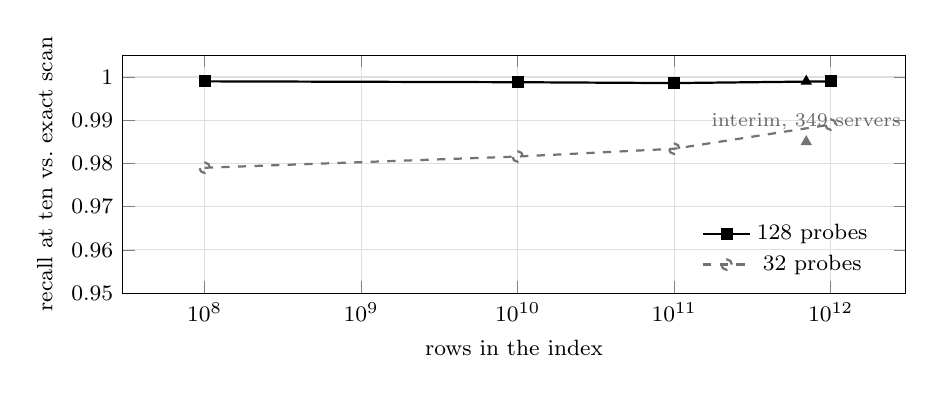
\begin{tikzpicture}
\begin{axis}[
  width=0.95\columnwidth, height=4.6cm,
  xmode=log, log basis x=10,
  xmin=3e7, xmax=3e12,
  ymin=0.95, ymax=1.005,
  xlabel={rows in the index},
  ylabel={recall at ten vs.\ exact scan},
  xtick={1e8,1e9,1e10,1e11,1e12},
  xticklabels={$10^{8}$,$10^{9}$,$10^{10}$,$10^{11}$,$10^{12}$},
  ytick={0.95,0.96,0.97,0.98,0.99,1.00},
  yticklabel style={/pgf/number format/fixed,/pgf/number format/precision=2},
  grid=major, grid style={gray!25},
  legend pos=south east, legend style={font=\footnotesize, draw=none, fill=none},
  tick label style={font=\footnotesize}, label style={font=\footnotesize},
]
\addplot[color=black, mark=square*, mark size=1.8pt, thick] coordinates {(1e8,0.999) (1e10,0.9988) (1e11,0.9986) (1e12,0.999)};
\addlegendentry{128 probes}
\addplot[color=black!55, mark=o, mark size=1.9pt, thick, dashed] coordinates {(1e8,0.979) (1e10,0.9816) (1e11,0.9834) (1e12,0.989)};
\addlegendentry{32 probes}
\addplot[color=black!55, mark=triangle*, mark size=2pt, only marks] coordinates {(6.98e11,0.985)};
\addplot[color=black, mark=triangle*, mark size=2pt, only marks] coordinates {(6.98e11,0.999)};
\node[font=\scriptsize, anchor=south, black!60] at (axis cs:6.98e11,0.9855) {interim, 349 servers};
\end{axis}
\end{tikzpicture}
\caption{Recall against the exact scan by corpus size. The triangles are the interim score taken
while the $10^{12}$ run was two thirds through its routed phase, on the 349 servers that had
finished both phases, 698 billion rows. They sit on the final points.}
\label{fig:scale}
\end{figure}

\subsection{Recall across four orders of magnitude}

Table~\ref{tab:scale} and Figure~\ref{fig:scale} give the number the run exists to produce. At
$10^{12}$ rows, routed search at 128 probes of 2048 cells returns 0.999 of the exact scan's top
ten, and at 32 probes 0.989. At 128 probes the figure is 0.999, 0.9988 and 0.9986 at the three
smaller scales, a spread of 0.0004. At 32 probes it rises slowly with scale, 0.979, 0.982, 0.983,
0.989, which is consistent with the merge over more servers filling the tail of the shortlist and
is not something we claim to explain. The interim score, taken on the first 349 servers to finish
both phases, gave 0.985 and 0.999, and recall at 128 probes on the first half of those 349
servers alone was also 0.999. The number is stable inside the run as well as across runs.

The $10^{9}$ row has no routed-versus-scan figure in the table because that run's purpose was
different. It carried a cold store of the original float vectors, so it measured true recall
against float ground truth. The routed shortlist at 128 probes returned 0.999 of the compressed
scan there too, the compressed scan itself found only 0.592 of the true neighbours, and reranking
the shortlist against the stored originals raised that to 0.991. That row is the reason
Section~\ref{sec:limits} exists.

\subsection{Cost}
\label{sec:cost}

\begin{table}[t]
\caption{Per-server wall time in the $10^{12}$ run, one CPU per job, 500 servers per phase, and
the CPU-hours each phase consumed.}
\label{tab:cost}
\centering
\small
\begin{tabular}{lrrrrr}
\toprule
phase & median & mean & p90 & max & CPU-h \\
\midrule
exact scan       & 2664 s & 3008 s & 4013 s & 16308 s & 418 \\
routed, 32       & 1064 s & 1131 s &        & 14286 s & 157 \\
routed, 128      & 1335 s & 1420 s &        & 14524 s & 197 \\
\bottomrule
\end{tabular}
\end{table}

Table~\ref{tab:cost} gives what the measurement cost. The exact scan of two billion rows at one
CPU takes 44 minutes at the median and the routed pass 18 to 22 minutes. Two things about these
numbers should be said plainly. First, the ratio between the routed and exact rows is not a
latency figure for the method. These jobs are read-bound on network block storage, spend a fixed
minute or two on image pull, dependency install and clone, and open 400 shards before scoring.
The $10^{11}$ run, on six CPUs per job, reported 14.7 and 8.5 as the same ratio, and neither
number is the method's. Second, the tails are the cluster's, not the index's. The 16308 s maximum
is one server on one node that also produced the slowest routed job, and the p90 is within 1.5 of
the median.

\section{Fitting the exempt envelope}
\label{sec:shape}

The platform enforces that a pod's usage sits within 20 to 200 percent of its CPU request and 20
to 150 percent of its memory request, averaged over minutes, and deletes pods that do not. Pods
requesting at most one CPU and two gigabytes are exempt. An earlier note in the repository records
that requests above two gigabytes were also deleted by a usage-independent rule in some windows,
so the exempt envelope is the only shape that is safe at all times on this cluster. The first
attempt at this measurement ran the exact scan at six CPUs and eight gigabytes. One pod metered at
8 percent of its CPU and 3 percent of its memory, another swung between 1.5 and 7.5 gigabytes over
its life, and a right-sizing tool the run carries scored the workload as having no legal request,
since a request must exceed the peak while a fifth of it must stay below the trough. The run was
stopped at 153 of 500 servers.

Three changes put the scan inside one CPU and two gigabytes. Each was found by a two-gigabyte
pilot that died without it, in this order.

\begin{enumerate}
\item \textbf{Queries from the cache.} The scan script derived its 100 queries by regenerating
four whole five-million-row blocks, about 640 MB each plus temporaries. The pilot was killed for
memory 85 seconds after start. The routed script already read the cached file, and the scan script now
does too.
\item \textbf{Two open shards.} A memory-mapped shard still materializes its row-id and tombstone
arrays, 45 MB per five-million-row shard, and the sharded index held 128 shards open by default,
5.8 GB across a full scan. The pilot was killed after 17 minutes, around the 45th shard, and this
is the 7.5 GB peak the right-sizer had seen on the eight-gigabyte jobs. The scan now holds two
shards open and the routed pass eight, with two worker threads.
\item \textbf{Blocks of 65536 rows.} The scoring block bounds the per-block temporaries to tens
of megabytes.
\end{enumerate}

With all three, the pilot scan finished in 1912 s with CPU averaging 884 millicores and peaking
at 979, memory averaging 1242 MiB and peaking at 1469, and a process resident set of 346 MB at the
end. The routed pilot finished in 36 minutes at 475 millicores average, memory averaging 1258 MiB
and peaking at 1568, resident set 165 MB. The memory above the resident set is clean page cache
from the mapped index, which the kernel reclaims under the limit rather than killing the process.
We observed the routed pod at the two-gigabyte limit with 224 MB anonymous and 1.9 GB file-backed,
and it completed. The exempt envelope is therefore not a constraint on the method. It is a
constraint on how the method is written, and the three items above are the whole of it.

The score job, which merges 1500 small partials, was submitted at two CPUs and four gigabytes and
was never created by the controller. Resubmitted at one CPU and two gigabytes it was created within
seconds and finished in minutes.

\section{Running a pool on a shared cluster}
\label{sec:pool}

The measurement was driven by a pool of at most twenty jobs in flight with no wave barrier,
checkpointed per phase, restartable, and able to adopt jobs already on the cluster after a
restart. Table~\ref{tab:pool} gives what it did over the two days after the resume. We describe the
rules because the counts are only meaningful against them.

\begin{table}[t]
\caption{The resumed run, 2026-09-25 18:01 UTC to 2026-09-27 08:59 UTC. Reference phase counts
exclude the 152 servers finished before the stop.}
\label{tab:pool}
\centering
\small
\begin{tabular}{lr}
\toprule
submissions & 928 \\
completions (348 scan, 500 routed, 1 score) & 849 \\
recycles, job failed & 75 \\
\quad of which bus error on one host & 24 \\
\quad node lost (exit 255) & 13 \\
\quad node unreachable, pod stuck & 13 \\
\quad container sandbox failure & 2 \\
recycles, pending past 45 minutes & 26 \\
jobs deferred by the controller and waited on & 1 \\
servers parked or given up & 0 \\
operator restarts of the driver & 0 \\
\bottomrule
\end{tabular}
\end{table}

\paragraph{Rules.} A job whose Kubernetes object reports success is done. A job whose object
reports failure is recycled, meaning its object is deleted and, after an exponential back-off from
two minutes to thirty, resubmitted, up to forty times before the server is parked and swept again
later. A job whose pod has not reached the running state 45 minutes after submission is recycled
the same way. A job submitted through the controller but not yet visible as an object is waited
on for ninety polls, one a minute, before it is treated as lost. A job running longer than sixteen
hours is treated as wedged.

\paragraph{The deferral rule.} The last rule but one was the lesson of the first attempt. The
submission controller defers creating a job while five of the namespace's jobs are pending or the
cluster is busy, and retries for up to about an hour. The first driver treated two polls without an
object as a vanished job and resubmitted, which queued a duplicate behind every deferred original.
When another group's GPU jobs began pending at 03:30 UTC, that turned 234 deferrals into 234
duplicate submissions and cut throughput from 20 servers an hour to 3. Ninety polls of patience
is the fix, and the resumed run needed it exactly once, for the score job.

\paragraph{Failure classes.} Two dominated. One host on the cluster killed every job placed on it
with a bus error within 3 to 13 minutes of start, after the block volume attached successfully.
Eleven placements in the first four hours, no survivors, retries elsewhere all finished, and the
cost over the first eight hours was about 130 slot-minutes out of 9600. We had no way to exclude a node from the
controller's job description and did not need one. The second class, pods pending past 45
minutes, turned out to be benign in every instance we checked, because the original pod had in
fact run and the retry found its output within minutes. That is what idempotent jobs buy.

\paragraph{Two interventions by hand.} Three scan pods became stuck terminating on nodes whose
kubelet had stopped answering, and one routed pod ran at 34 millicores for 97 minutes on a node
whose storage path was slow. The sixteen-hour wedge rule would have caught all four eventually. We
removed the pods by hand, the job controller replaced them, and the replacements finished in
minutes to an hour. A rule for pods terminating longer than thirty minutes belongs in the driver
and did not exist. We report this because the honest count of operator actions in a two-day run
is four pod deletions and one resubmission, not zero.

\paragraph{Provenance.} The job containers cloned the repository's default branch at run time, so
the scanning code moved as the branch moved. Twelve commits appear in pod logs across the run. The
two phase scripts came from a configuration map replaced once at the resume, and the merge and
score code did not change. Pinning the clone to a commit is the one change to the descriptor we
would make before running again.

\section{What the result does and does not show}
\label{sec:limits}

The claim is narrow and we want it read narrowly. Recall of the routed shortlist against the exact
scan of the same compressed index is flat from $10^{8}$ to $10^{12}$ rows. That is a statement
about the inverted-file layer, its shared coarse quantizer and its merge, and it says the routing
loses nothing the exact scan finds, at either probe width, when the corpus grows by adding shards.

It is not a statement about recall against the truth. The compressed scan at $10^{9}$ rows found
0.592 of the float neighbours, and on a real corpus of 15 million Cohere Embed v3 vectors the same
index found 0.693 of them by exact scan, 0.689 by routing at 256 probes, and 0.981 after reranking
the routed shortlist against stored originals. On that real corpus the routed shortlist returned
0.990 of the compressed scan at 256 probes, so the routing result transfers, and the compression
result does not. Four bits per dimension at this rate loses neighbours that only a rerank tier
recovers, and the trillion-row corpus, at intrinsic dimension 16 against a real embedding's 52 to
61, cannot show that. It is an easy corpus for the code and a hard one only for the hubness the
shards' overlap induces.

Two further limits. One hundred queries is few. The exact scan is compute-bound in the query
count and 500 queries would have cost about five times the 418 CPU-hours. And a cold store of
originals at $10^{12}$ rows would be 128 TB of float vectors, so true recall and reranking remain
established at $10^{9}$ and at the 15-million-row real pilot, not here.

\section{Related work}

Product quantization with asymmetric distance computation and inverted files is the basis of the
index \cite{jegou2011product}, and locally optimized codebooks per cell \cite{kalantidis2014lopq}
the nearest relative of the shared-basis arrangement we use to keep scores comparable across
shards. Faiss \cite{johnson2019faiss} established billion-scale practice on one machine, and
SPANN \cite{chen2021spann} the disk-resident inverted index at a billion rows. Graph indexes
\cite{malkov2020hnsw} are the usual alternative and are not what this paper measures. Hubness
\cite{radovanovic2010hubs} is the property of the corpus that does grow with scale here. What we
add is not a method but a measurement that the cited systems have not, to our knowledge,
published at this size against an exact scan of their own index, together with a complete account
of what it takes to obtain it on a shared cluster under usage enforcement.

\section{Conclusion}

A trillion-row compressed index can be built and measured exactly on a shared research cluster
with no reserved hardware, in the smallest resource class the platform offers, once three memory
paths are closed and a pool driver knows the difference between a deferred job and a lost one.
On that index, routing loses nothing the exact scan finds, at $10^{8}$ rows or at $10^{12}$. The
run cost 772 CPU-hours and two days, and it is entirely reproducible from the repository, which
carries the seeds, the scripts, the driver, the state files, both driver logs, the pilots, the
interim score and the final score with every per-server wall time.

\begin{acks}
This work used the National Research Platform's Nautilus cluster, supported by the National
Science Foundation, and we thank its operators for their patience with a two-day run in the
exempt class. The run was announced on the platform's community channel before launch.
\end{acks}

\bibliographystyle{ACM-Reference-Format}
\bibliography{refs}

\end{document}
